\documentclass[10pt]{article}
\usepackage[usenames]{color} %used for font color
\usepackage{amssymb} %maths
\usepackage{amsmath} %maths
\usepackage[utf8]{inputenc} %useful to type directly diacritic characters

%%% Sans serif text font
\usepackage[scaled]{helvet}
\renewcommand*\familydefault{\sfdefault}\usepackage[T1]{fontenc}
%%%

\usepackage[paperwidth=16in, paperheight=8in]{geometry}
\thispagestyle{empty}

\usepackage{skull}
\usepackage{tikz}
\usetikzlibrary{positioning}
\usetikzlibrary{arrows}
\usetikzlibrary{fit}
\usetikzlibrary{calc}
\usetikzlibrary{automata}
\usetikzlibrary{decorations.markings}
\usetikzlibrary{decorations.pathreplacing}
\usetikzlibrary{shapes.geometric}
\usetikzlibrary{external}

\tikzset{>=latex}
\tikzstyle{snode}=[black,draw=black,line width=1.5pt,shape=circle,fill=white,minimum size=8mm]
\tikzstyle{obnode}=[black,draw=black,line width=1.5pt,shape=circle,fill=black!20!white,minimum size=8mm]
\tikzstyle{detnode}=[black,draw=black,line width=1.5pt,densely dotted,shape=circle,fill=white,minimum size=8mm]
\tikzstyle{constnode}=[black,draw=black,line width=1.5pt,shape=rectangle,fill=white,minimum size=8mm]
\tikzstyle{distnode}=[black,draw=black,line width=1.5pt,shape=diamond,fill=white,minimum size=8mm]
\tikzstyle{mincnode}=[black,draw=black,line width=0.75pt,shape=rectangle,fill=white,minimum size=3mm]
\tikzstyle{blnode}=[white,draw=black,line width=1pt,shape=circle,fill=black,minimum size=1mm,font=\scriptsize,inner sep=1pt]
\tikzstyle{ylnode}=[black,draw=black,line width=1pt,shape=circle,fill=yellow,minimum size=1mm,font=\scriptsize,inner sep=1pt]
\tikzstyle{taro}=[->,line width=2pt,color=black]
\tikzstyle{thintaro}=[->,line width=0.75pt,color=black]
\tikzstyle{dtaro}=[->,line width=2pt, densely dotted,color=black]
\tikzstyle{smod}=[black, draw=black, line width=2pt, fill=white, shape=rectangle, rounded corners, minimum size=10mm, minimum width=20mm]
\tikzstyle{obmod}=[black, draw=black, line width=2pt, fill=black!20!white, shape=rectangle, rounded corners, minimum size=10mm, minimum width=20mm, minimum width=20mm]

\definecolor{shc}{RGB}{238,224,229}
\definecolor{shc2}{RGB}{182,152,195}
\definecolor{brnt}{RGB}{221,132,13}

\begin{document}

% \definecolor{shc}{RGB}{183,207,237}
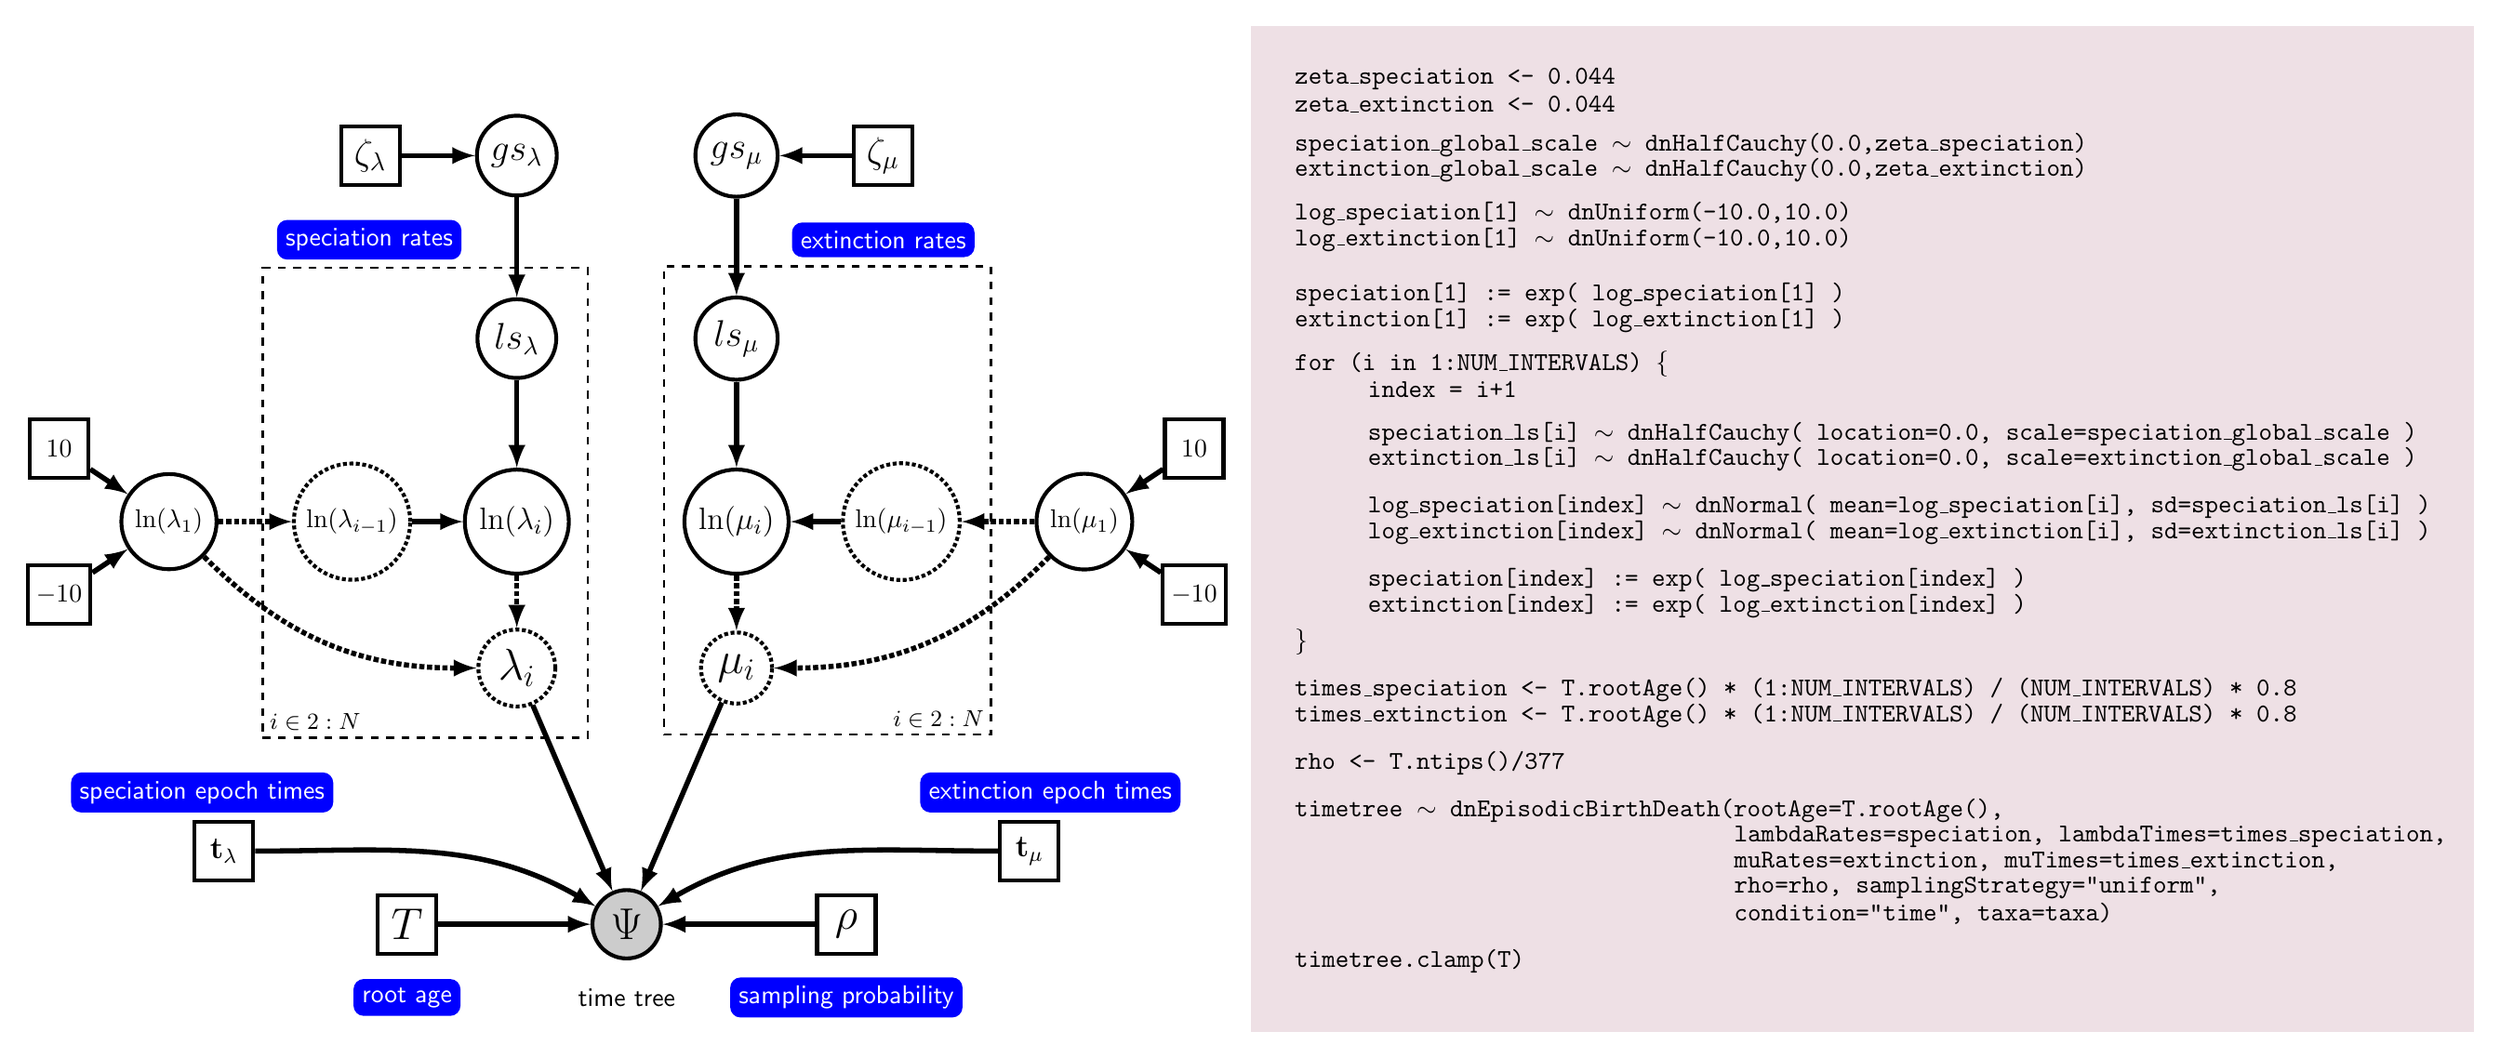
\begin{tikzpicture}
\node[obnode] (nx) at (1,1) {\LARGE $\Psi$};
\node[detnode] (lambda) at ($(nx)+(-1.5,3.5)$) {\LARGE $\lambda_{i}$};
\node[detnode] (mu) at ($(nx)+(1.5,3.5)$) {\LARGE $\mu_{i}$};
\node[snode] (ln_lambda) at ($(lambda)+(0,2.0)$) {\large $\ln(\lambda_{i})$};
\node[snode] (ln_mu) at ($(mu)+(0,2.0)$) {\large $\ln(\mu_{i})$};
\node[detnode] (lambda_prev) at ($(ln_lambda)-(2.25,0)$) {$\ln(\lambda_{i-1})$};
\node[detnode] (mu_prev) at ($(ln_mu)+(2.25,0)$) {$\ln(\mu_{i-1})$};
\node[snode] (lambda_init) at ($(lambda_prev)-(2.5,0)$) {$\ln(\lambda_{1})$};
\node[snode] (mu_init) at ($(mu_prev)+(2.5,0)$) {$\ln(\mu_{1})$};
\node[constnode] (lambda_init_min) at ($(lambda_init)+(-1.5,-1)$) {$-10$};
\node[constnode] (lambda_init_max) at ($(lambda_init)+(-1.5,1)$) {$10$};
\node[constnode] (mu_init_min) at ($(mu_init)+(1.5,-1)$) {$-10$};
\node[constnode] (mu_init_max) at ($(mu_init)+(1.5,1)$) {$10$};
\node[snode] (ls_lambda) at ($(ln_lambda)+(0,2.5)$) {\Large $ls_\lambda$};
\node[snode] (ls_mu) at ($(ln_mu)+(-0,2.5)$) {\Large $ls_\mu$};
\node[snode] (gs_lambda) at ($(ls_lambda)+(0,2.5)$) {\Large $gs_\lambda$};
\node[snode] (gs_mu) at ($(ls_mu)+(-0,2.5)$) {\Large $gs_\mu$};
\node[constnode] (gs_lambda_prior) at ($(gs_lambda)+(-2,0)$) {\Large $\zeta_\lambda$};
\node[constnode] (gs_mu_prior) at ($(gs_mu)+(2,0)$) {\Large $\zeta_\mu$};
\draw [taro] (lambda) -- (nx);
\draw [taro] (mu) -- (nx);
\draw [dtaro] (ln_lambda) -- (lambda);
\draw [dtaro] (ln_mu) -- (mu);
\draw [dtaro] (lambda_init) to [out=315,in=180] (lambda);
\draw [dtaro] (mu_init) to [out=225,in=0] (mu);
\draw [taro] (lambda_prev) -- (ln_lambda);
\draw [taro] (ls_lambda) -- (ln_lambda);
\draw [taro] (mu_prev) -- (ln_mu);
\draw [taro] (ls_mu) -- (ln_mu);
\draw [taro] (gs_mu) -- (ls_mu);
\draw [taro] (gs_lambda) -- (ls_lambda);
\draw [taro] (gs_mu_prior) -- (gs_mu);
\draw [taro] (gs_lambda_prior) -- (gs_lambda);
\draw [dtaro] (lambda_init) -- (lambda_prev);
\draw [taro] (lambda_init_min) -- (lambda_init);
\draw [taro] (lambda_init_max) -- (lambda_init);
\draw [dtaro] (mu_init) -- (mu_prev);
\draw [taro] (mu_init_min) -- (mu_init);
\draw [taro] (mu_init_max) -- (mu_init);
\node at ($(nx)+(0,-1)$) {time tree};
\node[constnode] (rho) at ($(nx)+(3,0)$) {\LARGE $\rho$};
\node[constnode] (T) at ($(nx)+(-3,0)$) {\LARGE $T$};
\node[constnode] (times_lambda) at ($(nx)+(-5.5,1)$) {\large $\mathbf{t}_\lambda$};
\node[constnode] (times_mu) at ($(nx)+(5.5,1)$) {\large $\mathbf{t}_\mu$};
\draw[taro] (T) -- (nx) ;
\draw[taro] (rho) -- (nx) ;
\draw [taro] (times_lambda) to [out=0,in=150] (nx);
\draw [taro] (times_mu) to [out=180,in=30] (nx);
\node[white, fill=blue, shape=rectangle, rounded corners] at ($(T)+(0,-1)$) {root age};
\node[white, fill=blue, shape=rectangle, rounded corners] at ($(rho)+(0,-1)$) {sampling probability};
\node[white, fill=blue, shape=rectangle, rounded corners] at ($(lambda_prev)+(1.5,3.85)$) [left]{speciation rates};
\node[white, fill=blue, shape=rectangle, rounded corners] at ($(mu_prev)+(-1.5,3.85)$) [right]{extinction rates};
\node[white, fill=blue, shape=rectangle, rounded corners] at ($(times_lambda)+(1.5,0.8)$) [left]{speciation epoch times};
\node[white, fill=blue, shape=rectangle, rounded corners] at ($(times_mu)+(-1.5,0.8)$) [right]{extinction epoch times};
\node[rectangle,dashed, thick, inner sep=4mm, draw=black!100, fit = (ls_lambda) (lambda_prev) (lambda)] (divPlate) {};
\node[rectangle,dashed, thick, inner sep=4mm, draw=black!100, fit = (ls_mu) (mu_prev) (mu)] (extPlate) {};
\node[anchor=south west,inner sep=3pt] at (divPlate.south west) {\small $i \in 2:N$};
\node[anchor=south east,inner sep=3pt] at (extPlate.south east) {\small $i \in 2:N$};
% %\node at ($(rho)+(-1.5,0)$) {Beta};
\node (a1) at (10.25,0.25) { };
\node (a2) at (10.25,12.55) { };
\node (a3) at (25.5,2.75) { };
\node[rectangle, very thick, inner sep=6mm, fill=shc, fit = (a1) (a2) (a3)] (console) {};
\node (l1) at (10.0,12.55) [right]{\tt zeta\_speciation <- 0.044};
\node (l2) at (10.0,12.2) [right]{\tt zeta\_extinction <- 0.044};
\node (l3) at (10.0,11.65) [right]{\tt speciation\_global\_scale $\sim$ dnHalfCauchy(0.0,zeta\_speciation)};
\node (l4) at (10.0,11.3) [right]{\tt extinction\_global\_scale $\sim$ dnHalfCauchy(0.0,zeta\_extinction)};
\node (l5) at (10.0,10.7) [right]{\tt log\_speciation[1] $\sim$ dnUniform(-10.0,10.0)};
\node (l6) at (10.0,10.35) [right]{\tt log\_extinction[1] $\sim$ dnUniform(-10.0,10.0)};
\node (l7) at (10.0,9.6) [right]{\tt speciation[1] := exp( log\_speciation[1] )};
\node (l8) at (10.0,9.25) [right]{\tt extinction[1] := exp( log\_extinction[1] )};
\node (l9) at (10.0,8.65) [right]{\tt for (i in 1:NUM\_INTERVALS) \{};
\node (l10) at (11.0,8.3) [right]{\tt index = i+1};
\node (l11) at (11.0,7.7) [right]{\tt speciation\_ls[i] $\sim$ dnHalfCauchy( location=0.0, scale=speciation\_global\_scale )};
\node (l11) at (11.0,7.35) [right]{\tt extinction\_ls[i] $\sim$ dnHalfCauchy( location=0.0, scale=extinction\_global\_scale )};
\node (l13) at (11.0,6.7) [right]{\tt log\_speciation[index] $\sim$ dnNormal( mean=log\_speciation[i], sd=speciation\_ls[i] )};
\node (l14) at (11.0,6.35) [right]{\tt log\_extinction[index] $\sim$ dnNormal( mean=log\_extinction[i], sd=extinction\_ls[i] )};
\node (l15) at (11.0,5.7) [right]{\tt speciation[index] := exp( log\_speciation[index] )};
\node (l16) at (11.0,5.35) [right]{\tt extinction[index] := exp( log\_extinction[index] )};
\node (l17) at (10.0,4.85) [right]{\tt \}};
\node (l18) at (10.0,4.20) [right]{\tt times\_speciation <- T.rootAge() * (1:NUM\_INTERVALS) / (NUM\_INTERVALS) * 0.8};
\node (l19) at (10.0,3.85) [right]{\tt times\_extinction <- T.rootAge() * (1:NUM\_INTERVALS) / (NUM\_INTERVALS) * 0.8};
\node (l20) at (10.0,3.20) [right]{\tt rho <- T.ntips()/377};
\node (l21) at (10.0,2.55) [right]{\tt timetree $\sim$ dnEpisodicBirthDeath(rootAge=T.rootAge(), };
\node (l22) at (16.0,2.20) [right]{\tt lambdaRates=speciation, lambdaTimes=times\_speciation, };
\node (l23) at (16.0,1.85) [right]{\tt muRates=extinction, muTimes=times\_extinction, };
\node (l24) at (16.0,1.5) [right]{\tt rho=rho, samplingStrategy="uniform", };
\node (l25) at (16.0,1.15) [right]{\tt condition="time", taxa=taxa)};
\node (l26) at (10,0.5) [right]{\tt timetree.clamp(T) };
\end{tikzpicture}

\end{document}
